\chapter{Interroger}
\minitoc

\section{Analyser}

Nous pouvons obtenir le modèle relationnel de la base de données par deux méthodes :

\begin{itemize}
    \item \textbf{PgAdmin 4 :} \textit{Clique Droit sur BDD/ ERD For DataBase}
    \item \textbf{DbSchema : } \textbf{Connect To DataBase/PostgreSQL/JDBC URL : Standard/Remote compunter/onglet : public}
\end{itemize}

\begin{figure} [H]
    \centering
    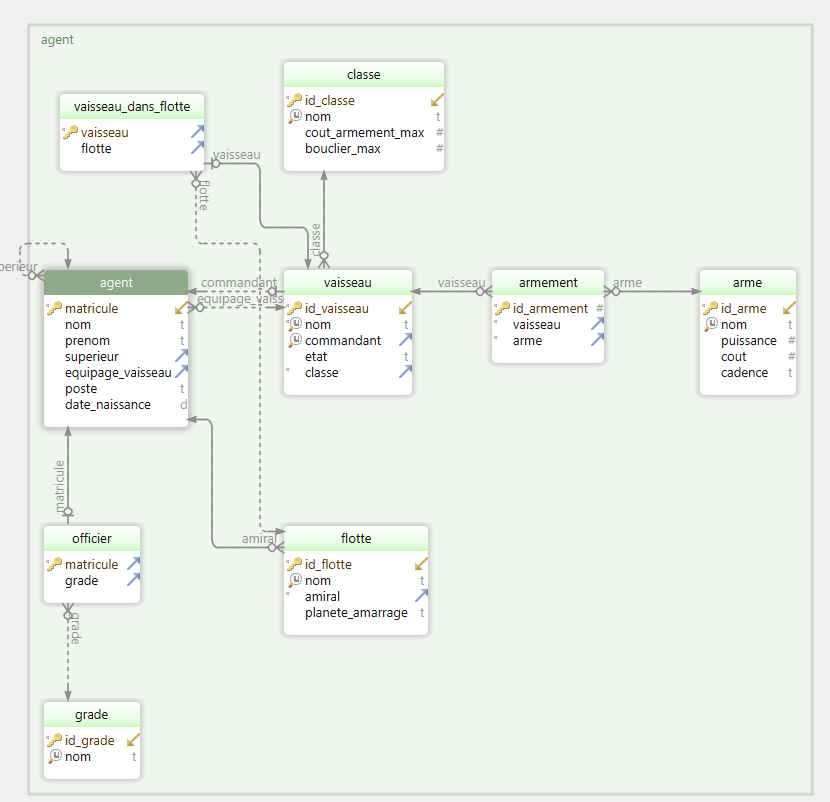
\includegraphics[width=0.8\linewidth]{image/MR_Seq4.png}
    \caption{MR BDD\_vaisseaux}
    \label{fig:enter-label}
\end{figure}


\section{Interrogation simple}

\subsection{Requête \texttt{SELECT}}
\begin{lstlisting}[language=SQL]
SELECT <attribut> FROM <table>
\end{lstlisting}

\subsection{Recherche par caractère}
Pour sélectionner l'ensemble des attributs commençant, terminant par une lettre ou contenant une lettre, on utilise \texttt{\%}
\begin{lstlisting}[language=SQL]
SELECT <attribut> FROM <table> WHERE <attribut> LIKE '%S'; //Finie par S
SELECT <attribut> FROM <table> WHERE <attribut> LIKE 'S%'; //Commence par S
SELECT <attribut> FROM <table> WHERE <attribut> LIKE '%S%'; //Contient S
\end{lstlisting}

\subsection{Combinaison}
Il est possible de combiner des requêtes, en effectuant une seconde requête dans une première
\begin{lstlisting}[language=SQL]
SELECT * FROM vaisseau IN (SELECT id_classe WHERE nom LIKE 'frégate')
\end{lstlisting}

\subsection{Rechercher dans une requête}
Il est possible de réaliser des requêtes dans des requêtes, notamment pour des agrégations (cf. §\ref{agregation})
\begin{lstlisting}[language=SQL]
SELECT 
    MAX(query_max.nbr_contenu)
FROM(
    SELECT
	COUNT(id_contenu) AS "nbr_contenu", 
	id_genre
    FROM contenu_genre 
    GROUP BY id_genre) AS query_max
\end{lstlisting}
\textbf{Attention} à bien utiliser un alias (cf. §\ref{allias})

\subsection{Afficher les tables de la BDD}
\begin{lstlisting}[language=SQL]
SELECT table_name
FROM information_schema.tables
WHERE table_schema = 'public';
\end{lstlisting}

\subsection{Afficher les attributs d'une table}
\begin{lstlisting}[language=SQL]
SELECT column_name, data_type
FROM information_schema.columns
WHERE table_name = 'nom_de_la_table';
\end{lstlisting}

\subsection{Compter le nombre de caractères}
LLa fonction \textbf{CHAR\_LENGTH()} permet de compter le nombre de caractères. On peut l'utiliser pour créer des conditions dans une requête. \textbf{Attention :} si la valeur de l'attribut est nulle, le test sera faux. Il faut donc tester si l'attribut est nul.
\begin{lstlisting}[language=SQL]
SELECT nom, prenom, poste FROM agent WHERE CHAR_LENGTH(prenom) <= 3 OR prenom IS NULL
\end{lstlisting}

\subsection{Trier par ordre alphabétique}
\texttt{ORDER BY} permet d'afficher les tuples souhaités dans un certain ordre. Par exemple ordre alphabétique croissant ou décroissant :
\begin{lstlisting}[language=SQL]
SELECT * FROM vaisseau ORDER BY nom ASC; //A->Z
SELECT * FROM vaisseau ORDER BY nom DESC; //Z->A
\end{lstlisting}

\subsection{Ne pas afficher les doublons}
\texttt{DISTINCT} permet d'afficher que les éléments distincts lors d'une requête.
\begin{lstlisting}[language=SQL]
SELECT DISTINCT poste FROM agent
\end{lstlisting}

\subsection{Compter les résultats}
\texttt{COUNT()} Permet de compter les résultats :
\begin{lstlisting}[language=SQL]
SELECT COUNT(*) FROM arme WHERE puissance <= 200
\end{lstlisting}

\subsection{Opérateurs de comparaison}
\begin{itemize}
    \item \texttt{LIKE} : Comparaison de texte non sensible à la casse
    \item \texttt{=} : Égal à
    \item \texttt{!=} : Différent de
    \item \texttt{\>, \>=, \<, \<=} : Supérieur à, supérieur ou égal à, inférieur à, inférieur ou égal à respectivement
    \item \texttt{NOT} : Négation
    \item \texttt{IS} : Permet de tester si attribut est nul et ou non nul
\end{itemize}
\textbf{ATTENTION :} Les comparaisons de texte doivent être effectuées entre apostrophes, par exemple, \texttt{'\<texte\>'}.


\subsection{Concaténer deux attributs}
\texttt{CONCAT()} permet de concaténer deux attributs dans une colonne lors d'une recherche, exemple :
\begin{lstlisting}[language=SQL]
SELECT CONCAT(prenom, nom) AS nom_agent FROM agent; --1ere syntaxe
SELECT prenom||nom AS nom_agent FROM agent; --2nd syntaxe
SELECT prenom||' '||nom AS nom_agent FROM agent; --Ajoute un espace
\end{lstlisting}

\subsection{Conversion en char}
Convertit l’expression d’entrée en chaîne. Pour une entrée NULL, la sortie est NULL

\subsubsection{Syntaxe}
\begin{lstlisting}[language=SQL]
TO_CHAR( <expr> ) --Une expression de tout type de données
TO_CHAR( <numeric_expr> [, '<format>' ] ) --Une expression numérique
TO_CHAR( <date_or_time_expr> [, '<format>' ] ) --Une expression de type DATE, TIME ou TIMESTAMP
TO_CHAR( <binary_expr> [, '<format>' ] ) --Une expression de type BINARY ou VARBINARY
\end{lstlisting}

\subsubsection{Exemples}
\begin{lstlisting}[language=SQL]
SELECT TO_CHAR('2013-04-05 01:02:03'::timestamp, 'MM/DD/YYYY, HH24:MI "hours"');

+--------------------------+
| 04/05/2013, 01:02 hours  |
+--------------------------+
\end{lstlisting}

\begin{lstlisting}[language=SQL]
SELECT TO_CHAR('03-May-2013'::date, 'YYYY-MM-DD');

+---------------------------------+
| TO_VARCHAR('03-MAY-2013'::DATE) |
|---------------------------------|
| 2013-05-03                      |
+---------------------------------+
\end{lstlisting}

\begin{lstlisting}[language=SQL]
SELECT TO_CHAR('03-May-2013'::date, 'yyyy.mm.dd');

+-----------------------------------------------+
| TO_VARCHAR('03-MAY-2013'::DATE, 'YYYY.MM.DD') |
|-----------------------------------------------|
| 2013.05.03                                    |
+-----------------------------------------------+
\end{lstlisting}

\begin{lstlisting}[language=SQL]
SELECT 
    column1 AS orig_value,
    to_char(column1, '$99.0') AS D2_1,
    to_char(column1, 'B9,999.0') AS D4_1,
FROM 
    (VALUES (-12.391), (0), (-1), (0.10), (0.01), (3987), (1.111)) AS t(column1);

+------------+--------+----------+
| ORIG_VALUE | D2_1     | D4_1   |
|------------+--------+----------+
|    -12.391 | -$12.4 |    -12.4 |
|      0.000 |   $0.0 |       .0 |
|     -1.000 |  -$1.0 |     -1.0 |
|      0.100 |   $0.1 |       .1 |
|      0.010 |   $0.0 |       .0 |
|   3987.000 |  $##.# |  3,987.0 |
|      1.111 |   $1.1 |      1.1 |
+------------+--------+----------+
\end{lstlisting}

\begin{lstlisting}[language = SQL]
SELECT TO_CHAR(54516, 'FM99999990D00')

+------------+-----------------+
| ORIG_VALUE | FM99999990D00   |
|------------+-----------------+
|    -54516  |         54516,00|
+------------+-----------------+
\end{lstlisting}

\textbf{ATTENTION :} Lors du copier/coller, les guillemets peuvent être modifiés.

\section{Jointures}

\subsection{Allias} \label{allias}
On utilise des allias pour simplifier la maintenance du code, on n'aura à modifier qu'un endroit le nom de table si son nom est modifié :
\begin{lstlisting}[language=SQL]
SELECT table.prenom AS firstname FROM agent AS table
\end{lstlisting}

\subsection{Jointures Internes}
On utilise des alias pour simplifier la maintenance du code ; ainsi, il n'y aura qu'un seul endroit à modifier si le nom de la table change :
\begin{figure}[H]
    \centering
    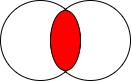
\includegraphics[width=0.25\linewidth]{image/INNER_JOIN.jpg}
    \caption{INNER JOIN}
    \label{fig:enter-label}
\end{figure}

La jointure interne en SQL :
\begin{lstlisting}[language=SQL]
SELECT
CONCAT(agent.nom, agent.prenom),
agent.matricule,
vaisseau.nom

FROM agent AS agent

INNER JOIN vaisseau AS vaisseau ON agent.equipage_vaisseau = vaisseau.id_vaisseau --Joint la seconde table
\end{lstlisting}

Autre exemple en ajoutant le trie de A à Z selon le nom de la flotte
\begin{lstlisting}[language=SQL]
SELECT
flotte.nom,
flotte.planete_amarrage,
agent.matricule AS matricule_amiral,
CONCAT(agent.prenom, agent.nom) AS amiral,
vaisseau.nom AS vaisseau_commandement

FROM flotte

INNER JOIN agent ON flotte.amiral = agent.matricule
INNER JOIN vaisseau ON agent.equipage_vaisseau = vaisseau.id_vaisseau

ORDER BY flotte.nom ASC
\end{lstlisting}

\subsection{Jointures externes}

\subsubsection{LEFT}
La jointure externe \texttt{LEFT} inclue la réunion des tables ainsi que la première table
\begin{figure}[H]
    \centering
    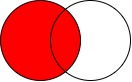
\includegraphics[width=0.25\linewidth]{image/LEFT.jpg}
    \caption{EXTERN LEFT}
    \label{fig:enter-label}
\end{figure}

Nous affichons ici les commandants associés à leurs vaisseaux et les agents,

\begin{lstlisting}[language=SQL]
SELECT 
v.nom, 
a.matricule, 
a.prenom||' '||a.nom

FROM agent AS a

LEFT JOIN vaisseau AS v ON a.matricule = v.commandant
\end{lstlisting}

\subsubsection{RIGHT}
La jointure externe \texttt{RIGHT} inclue la réunion des tables ainsi que la seconde table
\begin{figure}[H]
    \centering
    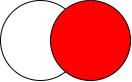
\includegraphics[width=0.25\linewidth]{image/RIGHT.jpg}
    \caption{EXTERN RIGHT}
    \label{fig:enter-label}
\end{figure}

Nous affichons ici les commandants associés à leurs vaisseaux et les agents,

\begin{lstlisting}[language=SQL]
SELECT 
v.nom, 
a.matricule, 
a.prenom||' '||a.nom

FROM vaisseau AS v

RIGHT JOIN agent AS a ON a.matricule = v.commandant
\end{lstlisting}

\subsubsection{FULL}
La jointure externe \texttt{FULL} inclue les deux tables
\begin{figure}[H]
    \centering
    
\includegraphics[width=0.25\linewidth]{image/FULL.jpg}
    \caption{EXTERN FULL}
    \label{fig:enter-label}
\end{figure}

\begin{lstlisting}[language=SQL]
SELECT 
attribut1

FROM table1

FULL JOIN table2 ON table1.attribut1 = table2.attribut25
\end{lstlisting}

\subsection{Utilisation des jointures}

\subsubsection{Plusieurs jointures}

On peut réaliser plusieurs jointures pour récupérer des attributs depuis plusieurs tables :
\begin{lstlisting}[language=SQL]
SELECT
flotte.nom,
flotte.planete_amarrage,
agent.matricule AS matricule_amiral,
CONCAT(agent.prenom, agent.nom) AS amiral,
vaisseau.nom AS vaisseau_commandement

FROM flotte

INNER JOIN agent ON flotte.amiral = agent.matricule
INNER JOIN vaisseau ON agent.equipage_vaisseau = vaisseau.id_vaisseau

ORDER BY flotte.nom ASC
\end{lstlisting}

\subsubsection{Table intermédiaire}

Nous pouvons utiliser des tables tempons pour réaliser une jointure entre deux tables qui ne sont pas directement liées par un attribut. Exemple :

\begin{lstlisting}[language=SQL]
SELECT
CONCAT(agent.nom, agent.prenom),
vaisseau.nom,
classe.nom

FROM agent

INNER JOIN vaisseau ON agent.equipage_vaisseau = vaisseau.id_vaisseau
INNER JOIN classe ON vaisseau.classe = classe.id_classe
\end{lstlisting}

\subsubsection{Conditions et trie}
Il est toujours possible d'ajouter des conditions ou de trier les tuples en plaçant les commandes après la jointure.

On réalise une jointure interne avec la table agent mais nous voulons une jointure externe gauche avec la table flotte
\begin{lstlisting}[language=SQL]
SELECT
v.nom AS nom_vaisseau,
a.matricule AS matricule_commandant,
a.nom AS nom_commandant,
f.nom AS nom_flotte

FROM vaisseau AS v

INNER JOIN agent AS a ON v.commandant = a.matricule --Jointure interne
LEFT JOIN vaisseau_dans_flotte AS vf ON vf.vaisseau = v.id_vaisseau --Jointure externe, table intermediaire
LEFT JOIN flotte AS f ON vf.flotte = f.id_flotte
\end{lstlisting}

\begin{lstlisting}[language=SQL]
SELECT
flotte.nom,
flotte.planete_amarrage,
agent.matricule AS matricule_amiral,
CONCAT(agent.prenom, agent.nom) AS amiral,
vaisseau.nom AS vaisseau_commandement

FROM flotte

INNER JOIN agent ON flotte.amiral = agent.matricule
INNER JOIN vaisseau ON agent.equipage_vaisseau = vaisseau.id_vaisseau

ORDER BY flotte.nom ASC
\end{lstlisting}

\section{Agrégations}\label{agregation}
\subsection{Définition}
Un agrégat est un partitionnement horizontal d'une table en sous-tables, en fonction des valeurs d'un ou plusieurs attributs de partitionnement, suivi éventuellement de l'application d'une fonction de calcul à chaque attribut des sous-tables obtenues. Les attributs définissant une sous table sous listé à la suite de \texttt{GROUP BY}. Exemple avec une moyenne sur les âges de personnes :

\begin{figure}[H]
    \centering
    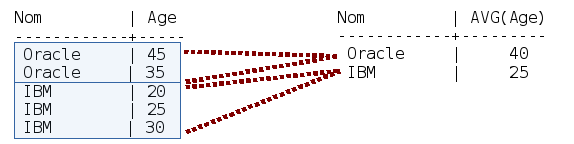
\includegraphics[width=0.7\linewidth]{image/regroupement-avec-fonction-0.png}
    \caption{Representation agrégation \texttt{Average}}
    \label{fig:enter-label}
\end{figure}

\subsection{Fonction \texttt{COUNT()}}
Renvoie le nombre de valeurs non nulles d'une propriété pour tous les tuples d'une relation, exemple :
\begin{lstlisting}[language=SQL]
SELECT
arme.nom,
COUNT (armement.id_armement)

FROM arme

INNER JOIN armement ON arme.id_arme = armement.arme

GROUP BY arme.nom
\end{lstlisting}

\begin{lstlisting}[language=SQL]
SELECT
f.nom,
COUNT (vf.vaisseau)

FROM flotte AS f

INNER JOIN vaisseau_dans_flotte AS vf ON f.id_flotte = vf.flotte

GROUP BY f.nom
\end{lstlisting}

\subsection{Conditions}
Pour rajouter une condition sur un agrégation on utilie le key word \texttt{HAVING}, exemple :

\begin{lstlisting}[language=SQL]
SELECT
arme.nom,
COUNT (armement.id_armement)

FROM arme

INNER JOIN armement ON arme.id_arme = armement.arme

GROUP BY arme.nom

HAVING
    COUNT (armement.id_armement) > 100
\end{lstlisting}

\subsection{Fonction \texttt{MAX()}}
Renvoie la plus grande valeur d'une propriété parmi les tuples d'une relation, exemple : 

\begin{lstlisting}[language = SQL]
SELECT
v.nom,
MAX(a.puissance)

FROM vaisseau AS v

INNER JOIN armement AS ar ON ar.vaisseau=v.id_vaisseau
INNER JOIN arme AS a ON ar.arme = a.id_arme

GROUP BY v.nom

ORDER BY v.nom ASC
\end{lstlisting}

\subsection{Fonction \texttt{MIN()}}
Renvoie la plus petite valeur d'une propriété parmi les tuples d'une relation, exemple : 

\begin{lstlisting}[language = SQL]
SELECT
v.nom,
CONCAT(TO_CHAR(MIN(a.puissance),'FM99999990D00'),'MJ') AS puissance

FROM vaisseau AS v

INNER JOIN armement AS ar ON ar.vaisseau=v.id_vaisseau
INNER JOIN arme AS a ON ar.arme = a.id_arme

GROUP BY v.nom

ORDER BY v.nom ASC
\end{lstlisting}

\subsection{Fonction \texttt{SUM()}}
Renvoie la somme des valeurs d'une propriété des tuples (numériques) d'une relation, exemple :

\begin{lstlisting}[language=SQL]
SELECT
v.nom,
CONCAT(TO_CHAR(SUM(arme.puissance), 'FM99999990D00'),'MJ') AS somme_puissance

FROM vaisseau AS v

INNER JOIN armement ON armement.vaisseau = v.id_vaisseau
INNER JOIN arme ON arme.id_arme = armement.arme

GROUP BY v.nom
\end{lstlisting}

\subsection{Fonction \texttt{AVG()}}
Renvoie la moyenne des valeurs d'une propriété des tuples (numériques) d'une relation

\begin{lstlisting}[language=SQL]
SELECT
v.nom,
CONCAT(TO_CHAR(AVG(arme.puissance), 'FM99999990D00'),'MJ') AS moyenne_puissance

FROM vaisseau AS v

INNER JOIN armement ON armement.vaisseau = v.id_vaisseau
INNER JOIN arme ON arme.id_arme = armement.arme

GROUP BY v.nom
\end{lstlisting}

\subsection{Fonction \texttt{STRING\_AGG()}}
La fonction d'agrégation \texttt{STRING\_AGG()} est utilisée pour concaténer les valeurs de plusieurs lignes d'une colonne en une seule chaîne de caractères, en les séparant par un délimiteur spécifié. C'est particulièrement utile lorsqu'on souhaite agréger des valeurs d'une colonne en une seule chaîne de caractères pour un affichage ou un traitement ultérieur.

\begin{lstlisting}[language=SQL]
SELECT
  p.nom_libre AS "Nom Plateforme",
  MIN(d.date_diffusion) AS "Date Diffusion La Plus Ancienne",
  STRING_AGG(c.nom_libre, ', ') AS "Noms Contenus" --On veut les noms des éléments diffusés MIN
  
FROM plateforme AS p

INNER JOIN diffusion AS d ON d.id_plateforme = p.id
INNER JOIN contenu AS c ON d.id_contenu = c.id

GROUP BY p.nom_libre;   
\end{lstlisting}

\section{Exemple de requêtes}

\subsection{Multiples jointures}
\begin{lstlisting}[language=SQL]
SELECT
CONCAT(a.nom, ' ', a.nom) AS agent,
a.matricule AS "matricule agent",
ga.nom AS "grade agent",
CONCAT(s.nom, ' ', s.nom) AS superieur,
s.matricule AS "matricule superieur",
gs.nom AS "grade superieur"

FROM agent AS a

--Recupere le grade de l'agent
LEFT JOIN officier AS oa ON oa.matricule = a.matricule
LEFT JOIN grade AS ga ON ga.id_grade = oa.grade

--Recupere le superieur de l'agent
LEFT JOIN agent AS s ON a.superieur = s.matricule

--Recupere le grade du superieur
LEFT JOIN officier AS os ON os.matricule = s.matricule
LEFT JOIN grade AS gs ON gs.id_grade = os.grade
\end{lstlisting}

\begin{lstlisting}[language=SQL]
SELECT
v.nom AS "Nom Vaisseau",
c.nom AS "Classe",
f.nom AS "Flotte",
CONCAT (a.nom, ' ',a.prenom) AS "Commadandant",
a.matricule AS "Matricule Commandant",
g.nom AS "Grade Commandant"

FROM vaisseau AS v

--Recupere Classe
INNER JOIN classe AS c ON v.classe = c.id_classe

--Recupere Flotte
INNER JOIN vaisseau_dans_flotte AS vf ON vf.vaisseau = v.id_vaisseau
INNER JOIN flotte AS f ON f.id_flotte = vf.flotte

--Recupere Commandant
INNER JOIN agent AS a ON v.commandant = a.matricule

--Recupere Grade du commandant
INNER JOIN officier AS o ON o.matricule = a.matricule
INNER JOIN grade AS g ON g.id_grade = o.grade
\end{lstlisting}

\subsection{Agrégation et Jointures}
\begin{lstlisting}[language=SQL]
SELECT
v.nom AS "Vaisseau",
arme.nom AS "Arme",
COUNT (arme.nom) AS "Quantite de l arme"

FROM vaisseau AS v

INNER JOIN armement AS ar ON ar.vaisseau = v.id_vaisseau
INNER JOIN arme ON ar.arme = arme.id_arme

GROUP BY v.nom, arme.nom
\end{lstlisting}

\section{Vues}
Une vue dans une base de données est une synthèse d'une requête d'interrogation de la base. On peut la voir comme une table virtuelle, définie par une requête.

Les avantages des vues sont :

\begin{itemize}
    \item Eviter de taper une requête très longue : la vue sert à donner un nom à la requête pour l'utiliser souvent
    \item Masquer certaines données à certains utilisateurs. En SQL, les protections d'une vue ne sont pas forcément les mêmes que celles des tables sous-jacentes.
\end{itemize}

Exemple de vue :
\begin{lstlisting}[language=SQL]
CREATE VIEW vue_contenu_genre_type AS
SELECT
 c.nom_libre AS "contenu",
 c.date_creation,
 c.synopsis,
 tc.nom_libre AS "type_contenu",
 g.nom_libre AS "genre"
 
 FROM contenu AS c
 
 LEFT JOIN type_contenu AS tc ON c.id_type_contenu = tc.id
 LEFT JOIN contenu_genre AS cg ON cg.id_contenu = c.id
 LEFT JOIN genre AS g ON g.id = cg.id_genre
\end{lstlisting}